\documentclass{techbrief}

\usepackage{tikz, pgfplots}
\usetikzlibrary{positioning,calc,arrows,arrows.meta, shapes, decorations.markings}
\usetikzlibrary{decorations.pathreplacing}

\title{Non-linear representations in quantum mechanics}
\author{Gabriele Carcassi}
\category{Quantum mechanics}
\tags{Hilbert space, Projective space, collinear maps}

\begin{document}
	
\maketitle
	
\begin{abstract}
	The linear representation of quantum theory in terms of vector spaces is not a physical requirement but a convenient mathematical representation. We show this by providing a non-linear map that preserves the Born rule, and therefore all the physics.
\end{abstract}

\section{Introduction}

It is often stated that the linearity of quantum mechanics is a critical part of the theory. Here we show that the linearity of the vector space is not actually part of the physical requirements, and one can represent quantum theory with different vector spaces that are linked by a non-linear function. This means that the linearity of the vector space is more a convenient choice of representation than a physically meaningful requirement.

\section{Conditions}

We can sum up the definitions of a state space in quantum mechanics with the following condition.
\begin{condition}[Quantum states]{QST}
	The state space of the system is represented by a complex projective space $P(\mathcal{H})$. That is, a state $\psi \in P(\mathcal{H})$ is a ray $\psi = \{c |\psi\> \mid c \in \mathbb{C} \setminus \{ 0\} \}$ of some complex vector space $\mathcal{H}$. The conditional probability $p( \cdot \mid \cdot) : P(\mathcal{H}) \times P(\mathcal{H}) \to [0,1]$ is given by the Born rule. That is, $\mathcal{H}$ is equipped with an inner product such that $p(\psi|\phi) = \frac{\< \phi | \psi \>\< \psi | \phi \>}{\< \psi | \psi \>\< \phi | \phi \>}$.
\end{condition}
Note that the specific $\mathcal{H}$ is not considered part of the definition. The only requirement is that a suitable $\mathcal{H}$ exists.

The following condition associates the system with a specific space $\mathcal{H}$, which is now part of the specification.
\begin{condition}[Linear vector space representation]{REP-VSLIN}
	The system is associated with a complex inner product space $\mathcal{H}$, the state space is its projectivization and the Born rule is defined from its inner product.
\end{condition}

\section{Theorem}

\begin{thrm}[Linearity is a choice]
	Condition \ref{REP-VSLIN} is independent of \ref{QST}. That is, both \ref{REP-VSLIN} and $\neg$\ref{REP-VSLIN} are consistent with \ref{QST}.
\end{thrm}

\begin{proof}
	Since \ref{QST} states that the state space is the projectivization of some complex inner product space $\mathcal{H}$, \ref{REP-VSLIN} is trivially consistent with \ref{QST}.
	
	To prove $\neg$\ref{REP-VSLIN} is consistent with \ref{QST}, it suffices to show that there exists a non-linear map $m : \mathcal{H} \to \mathcal{H}$ that preserves the Born rule and maps rays to rays. Since the map is non-linear, $\mathcal{H} \nequiv m(\mathcal{H})$ in the category of vector spaces. However, since rays and Born rule are preserved, states and measurement outcomes can be represented by $m(\mathcal{H})$, and therefore the state space of the system is not the projectivization of a particular vector space.
	
	Consider a two-state system and let $|z^+\>$ and $|z^-\>$ be two orthonormal state vectors. Every vector in the Hilbert space can be expressed as a linear combination $|\psi\> = c_{+} | z^+ \> + c_{-} | z^- \>$. Now consider the map $m : \mathcal{H} \to \mathcal{H}$ defined by $m(0) \mapsto 0$ and, on non-zero vectors, by
	\begin{equation}
		\begin{aligned}
			m(c_{+} | z^+ \> + c_{-} | z^- \>) \mapsto e^{\imath \theta \frac{|c_{+}|^2}{|c_{+}|^2+|c_{-}|^2}} ( c_{+} | z^+ \> + c_{-}  | z^- \>),
		\end{aligned}
	\end{equation}
	where $\theta \in (0,2\pi)$ is an arbitrary constant. Note that $\frac{|c_{+}|^2}{|c_{+}|^2+|c_{-}|^2} = p(z^+|\psi)$ is the probability of measuring $z^+$ given the state $\psi$. On the Bloch ball, if we put $z^-$ at the bottom and $z^+$ at the top, the expression gives us the normalized vertical height from the bottom to the top of the sphere as seen in Fig. \ref{rp-qm-figNonLinear}. The map is therefore introducing a phase shift that depends on the vertical position.

\begin{figure}[h]
	\centering
	
	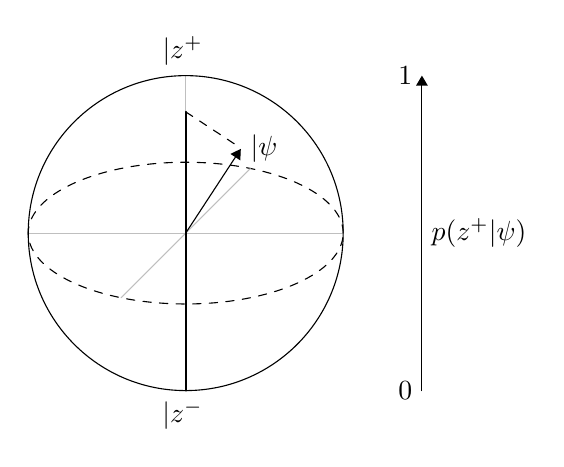
\begin{tikzpicture}[scale = 1.0, line cap=round, line join=round, >=Triangle]
		% equator
		\draw [rotate around={0.:(0.,0.)},dash pattern=on 3pt off 3pt] (0,0) ellipse (2cm and 0.9cm);
		% axis
		\draw [lightgray] (0,-2) -- (0,2);
		\draw [lightgray] (0.82,0.82) -- (-0.82,-0.82);
		\draw [lightgray] (-2,0) -- (2,0);
		% main circle
		\draw(0,0) circle (2cm);
		\draw [->] (0,0) -- (0.70,1.07);
		\draw [dashed] (0,1.54) -- (0.7,1.08);
		\draw [thick] (0,-2) -- (0,1.54);
		% symbols
		\draw (0.70,1.07) node[right] {$|\psi\>$};
		\draw (0,2) node[above] {$|z^+\>$};
		\draw (0,-2) node[below] {$|z^-\>$};
		\draw [->] (3,-2) -- node[right] {$p(z^+|\psi)$} (3,+2);
		\draw (3,-2) node[left] {$0$};
		\draw (3,2) node[left] {$1$};
		
		%\draw (0.4,1.65) node[anchor=north west] {$|\psi\>$};
		% decoration
		\scriptsize
		%\draw [fill] (0,0) circle (1.5pt);
		%\draw [fill] (0.7,1.1) circle (0.5pt);
	\end{tikzpicture} 
	\caption{\label{rp-qm-figNonLinear}Probability is vertical height on the Bloch sphere.}
\end{figure}

We verify that $m$ maps a ray to another ray. That is:
\begin{equation}
	\begin{aligned}
		m(k(c_{+} | z^+ \> + c_{-} | z^- \>)) &= m(kc_{+} | z^+ \> + k c_{-} | z^- \>) = e^{\imath \theta \frac{|kc_{+}|^2}{|kc_{+}|^2+|kc_{-}|^2}} ( k c_{+} | z^+ \> + k c_{-}  | z^- \>) \\
		&= k e^{\imath \theta \frac{|k|^2|c_{+}|^2}{|k|^2(|c_{+}|^2+|c_{-}|^2)}} ( c_{+} | z^+ \> + c_{-}  | z^- \>) = k e^{\imath \theta \frac{|c_{+}|^2}{|c_{+}|^2+|c_{-}|^2}} \left( c_{+} | z^+ \> + c_{-}  | z^- \> \right) \\
		&= k \, m(c_{+} | z^+ \> + c_{-} | z^- \>) \\
	\end{aligned}
\end{equation}
In fact, we can see that each ray is mapped to the same ray. We verify that the map is not linear. In fact:
\begin{equation}
	\begin{aligned}
		m(|z^+\>) &= e^{\imath \theta} |z^+\> \\
		m(|z^-\>) &= | z^- \>\\
		m(|z^+\> + |z^-\>) &= e^{\frac{\imath \theta}{2}}( |z^+\> +  | z^- \>) \neq m(|z^+\>) + m(|z^-\>) = e^{\imath \theta} |z^+\> + | z^- \>.
	\end{aligned}
\end{equation}

To verify the Born rule, let us first calculate how the inner product changes.
\begin{equation}
	\begin{aligned}
		\<m(v) | m(w) \> &= e^{-\imath \theta \frac{|v_{+}|^2}{|v_{+}|^2+|v_{-}|^2}} e^{\imath \theta \frac{|w_{+}|^2}{|w_{+}|^2+|w_{-}|^2}} \< v | w \>,
	\end{aligned}
\end{equation}
The inner product is manifestly not conserved. However, for the Born rule we have:
\begin{equation}
	\begin{aligned}
		\<m(v) | m(v) \> &= e^{-\imath \theta \frac{|v_{+}|^2}{|v_{+}|^2+|v_{-}|^2}} e^{\imath \theta \frac{|v_{+}|^2}{|v_{+}|^2+|v_{-}|^2}} \< v | v \> = \< v | v \> \\
		p(m(v)|m(w)) &= \frac{\< m(v) | m(w) \>\< m(w) | m(v) \>}{\< m(v) | m(v) \>\< m(w) | m(w) \>} \\
		&= \frac{e^{-\imath \theta \frac{|v_{+}|^2}{|v_{+}|^2+|v_{-}|^2}} e^{\imath \theta \frac{|w_{+}|^2}{|w_{+}|^2+|w_{-}|^2}} \< v | w \> e^{-\imath \theta \frac{|w_{+}|^2}{|w_{+}|^2+|w_{-}|^2}}e^{\imath \theta \frac{|v_{+}|^2}{|v_{+}|^2+|v_{-}|^2}}  \< w | v \>}{\< v | v \>\< w | w \>} \\
		&= \frac{\< v | w \>\< w | v \>}{\< v | v \>\< w | w \>} = p(v|w).
	\end{aligned}
\end{equation}
The Born rule is conserved even though the inner product is not.
\end{proof}

\begin{remark}
We should also note that $m$ is not just a bijective map, but also a diffeomorphism. This means that every other relationship in quantum mechanics can be expressed in this non-linear space through $m$. This includes superposition relationships, expectation of observables and time evolution. These relationships would become considerably more complicated for likely no benefit. Therefore, the fact that we use an underlying linear vector space is, technically, not a physical requirement: it's mathematical convenience.
\end{remark}

\section{Conclusion}

We have shown that non-linear maps that do not conserve the inner product but preserve the Born rule, and thus all the physics, exist and therefore the linear representation amounts to a choice of representation. We should also note that alternative representations exist that are not even tied to vector spaces: the Madelung equations (also known as the equations of quantum hydrodynamics) provide such a representation.

\end{document}
